\subsection{The Action Language $\AL$}

Simply put, action languages are a family of declarative languages designed for the purpose of describing the effects of actions. They have a simple syntax and semantics, while remaining powerful enough to represent many complex reasoning domains \cite{Bald2005}. Collections of statements are called \emph{action descriptions}, and define transitions whose nodes correspond to \emph{possible states of the world}\footnote{A difference we believe to be significant from the conception of a state in the classical view as simply an interpretation of the fluents present in a domain.}, and whose arcs are labeled by actions. An arc $\triple{\sigma}{\alpha}{\tau}$ states that if action $\alpha$ occurs in state $\sigma$, the resulting state will be $\tau$. In addition to specifying what changes due to the occurrence of a particular action, it is also vital to be able to specify what does not change. This is know as the \emph{frame problem} \cite{Shan97}, and its solution lies in an elegant and precise representation of what is called the \emph{inertia axiom}. The beauty and utility of such languages stems from the ability to compactly represent huge transition systems, and in their graceful approach towards solving the frame problem.

Action descriptions in the language of $\AL$ are collections of three statement types: \emph{dynamic causal laws}, \emph{static causal laws}, and \emph{impossibility conditions}. Dynamic causal laws are statements of the form:
\begin{align*}
    &\dynamiclawp{a}{f}{l_{0},\ldots,l_{n}}
\end{align*}
where $a$ is an action, and $f$, and $l_{0},\ldots,l_{n}$ are fluent literals. Laws of this form a read as: ``action $a$ causes $f$ to be come true if $l_{0},\ldots,l_{n}$.'' The corresponding arc in the transition diagram is shown in Figure~\ref{fig-dcl}.
\begin{figure}
    \centering
    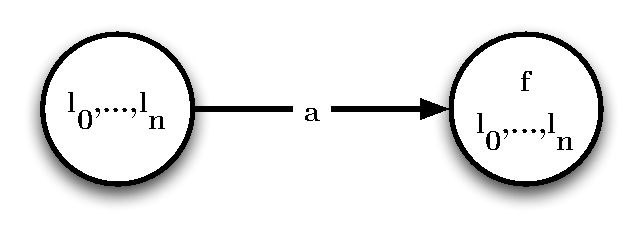
\includegraphics[scale=0.5]{dynamic-law}
    \caption{transition defined by a simple causal law}
    \label{fig-dcl}
\end{figure}

Static causal laws have the form:
\begin{align*}
    &\staticlaw{f}{l_{0},\ldots,l_{n}}
\end{align*}
where $f$, and $l_{0},\ldots,l_{n}$ are fluent literals. Such laws are read as: ``$f$ is true whenever $l_{0},\ldots,l_{n}$ are true.'' Unlike dynamic causal laws, static laws are used to describe the properties of states, as well as the \emph{indirect effects} of actions.
\begin{example}
{\rm
Consider the following action description $AD_{1}$:
\begin{align*}
    &\dynamiclaw{a}{f} \\
    &\staticlaw{g}{f}
\end{align*}
and let the state, $\sigma = \{\neg{f}, \neg{g}\}$. If $a$ is executed in $\sigma$, we have the transition depicted in Figure~\ref{fig-scl}.
\begin{figure}
    \centering
    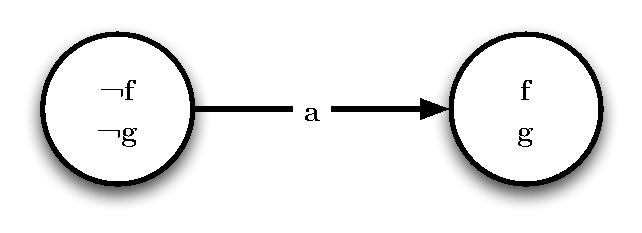
\includegraphics[scale=0.5]{static-law}
    \caption{transition involving both direct and indirect effects}
    \label{fig-scl}
\end{figure}
}
\end{example}

Impossibility conditions have the form:
\begin{align*}
    &\impossible{a}{l_{0},\ldots,l_{n}}
\end{align*}
where as before, $a$ is an action, and $l_{0},\ldots,l_{n}$ are fluent literals. Rules such as this are used to state that: ``action $a$ may not occur in a state which satisfies $l_{0},\ldots,l_{n}$.'' From the view of a transition system, this means that there are no outgoing arcs labeled by $a$ originating from a state which satisfies $l_{0},\ldots,l_{n}$.

The semantics of an action description of $\AL$ is given by its transition diagram. For a more detailed treatment, we refer the reader to \cite{Bald2005}.